% Author: Izaak Neutelings (July 2018)
\documentclass[border=3pt,tikz]{standalone}
\usepackage{amsmath}
\usepackage{tikz}
\usepackage{physics}
\tikzset{>=latex} % for LaTeX arrow head
%\usepackage{xcolor}
%\colorlet{force}{orange!80!black}
\tikzstyle{charge}=[thin,top color=red!50,bottom color=red!70,shading angle=20]
\tikzstyle{charge+}=[thin,top color=red!50,bottom color=red!90!black,shading angle=20]
\tikzstyle{charge-}=[thin,top color=blue!50,bottom color=blue!80,shading angle=20]
\tikzstyle{force}=[->,very thick,orange!80!black]
\tikzstyle{vector}=[->,very thick,green!45!black]
\def\a{2.5}
\def\R{0.33}
\def\F{1.8}


\begin{document}
\Large



% REPELLING CHARGES +q +q
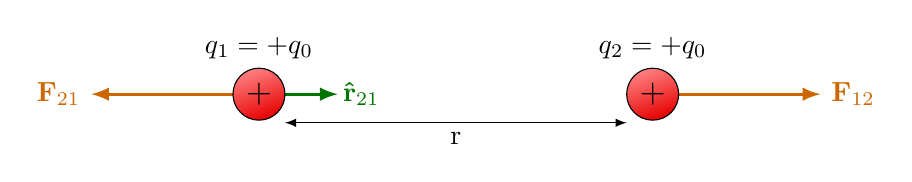
\begin{tikzpicture}
  \coordinate (L) at (-\a,0);
  \coordinate (R) at (+\a,0);
  
  % FORCES
  \draw[force] (L) ++ (-\R,0) --++ (-\F,0) node[left] {$\mathbf{F}_{21}$};
  \draw[force] (R) ++ (+\R,0) --++ (+\F,0) node[right] {$\mathbf{F}_{12}$};
  
  % POSITION VECTOR
  \draw[vector] (L) --++ (0.4*\a,0) node[right=-2] {$\vu{r}_{21}$};
  
  % CHARGES
  \draw[charge+] (L) circle (\R) node[scale=1.2] {$+$};
  \draw[charge+] (R) circle (\R) node[scale=1.2] {$+$};
  \draw[<->]     (L)++(\R,-1.1*\R) --++ (2*\a-2*\R,0) node[midway,below] {r};
  \node[above] at (-\a,\R) {$q_1=+q_0$};
  \node[above] at (+\a,\R) {$q_2=+q_0$};
  
\end{tikzpicture}


% REPELLING CHARGES  +2q +q
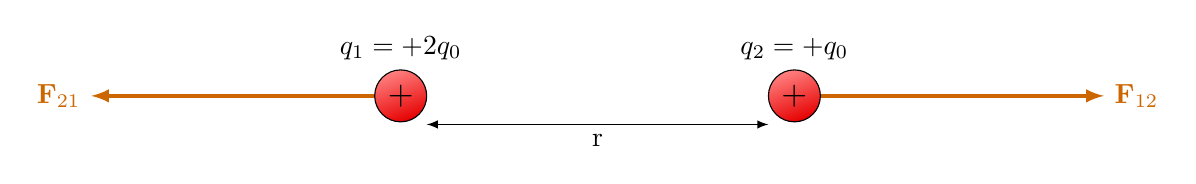
\begin{tikzpicture}
  \coordinate (L) at (-\a,0);
  \coordinate (R) at (+\a,0);
  
  % FORCES
  \draw[force] (L) ++ (-\R,0) --++ (-2*\F,0) node[left] {$\mathbf{F}_{21}$};
  \draw[force] (R) ++ (+\R,0) --++ (+2*\F,0) node[right] {$\mathbf{F}_{12}$};
  
  % CHARGES
  \draw[charge+] (L) circle (\R) node[scale=1.2] {$+$};
  \draw[charge+] (R) circle (\R) node[scale=1.2] {$+$};
  \draw[<->]     (L)++(\R,-1.1*\R) --++ (2*\a-2*\R,0) node[midway,below] {r};
  \node[above] at (-\a,\R) {$q_1=+2q_0$};
  \node[above] at (+\a,\R) {$q_2=+q_0$};
  
\end{tikzpicture}


% REPELLING CHARGES  +q +q, r' = 2r
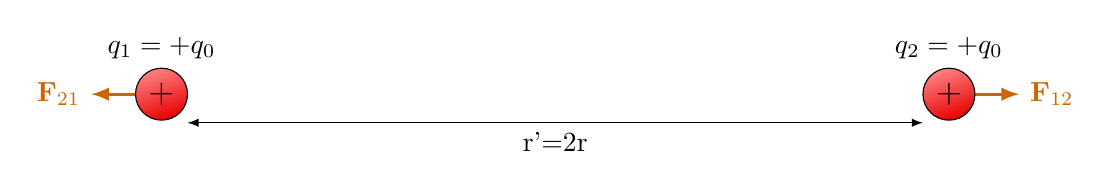
\begin{tikzpicture}
  \coordinate (L) at (-2*\a,0);
  \coordinate (R) at (+2*\a,0);
  
  % FORCES
  \draw[force] (L) ++ (-\R,0) --++ (-\F/3.2,0) node[left] {$\mathbf{F}_{21}$};
  \draw[force] (R) ++ (+\R,0) --++ (+\F/3.2,0) node[right] {$\mathbf{F}_{12}$};
  
  % CHARGES
  \draw[charge+] (L) circle (\R) node[scale=1.2] {$+$};
  \draw[charge+] (R) circle (\R) node[scale=1.2] {$+$};
  \draw[<->]     (L)++(\R,-1.1*\R) --++ (4*\a-2*\R,0) node[midway,below] {r'=2r};
  \node[above] at (-2*\a,\R) {$q_1=+q_0$};
  \node[above] at (+2*\a,\R) {$q_2=+q_0$};
  
\end{tikzpicture}



% ATTRACTING CHARGES
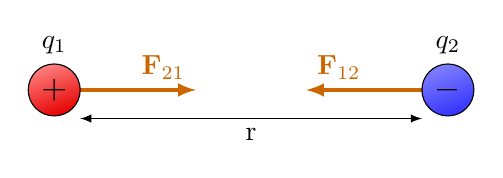
\begin{tikzpicture}
  \def\a{2.5}
  \coordinate (L) at (-\a,0);
  \coordinate (R) at (+\a,0);
    
  % FORCES
  \draw[force] (L) --++ (+\F,0) node[above left] {$\mathbf{F}_{21}$};
  \draw[force] (R) --++ (-\F,0) node[above right] {$\mathbf{F}_{12}$};
  
  % CHARGES
  \draw[charge+] (L) circle (\R) node[scale=1.2] {$+$};
  \draw[charge-] (R) circle (\R) node[scale=1.2] {$-$};
  \draw[<->]     (L)++(\R,-1.1*\R) --++ (2*\a-2*\R,0) node[midway,below] {r};
  \node[above] at (-\a,\R) {$q_1$};
  \node[above] at (+\a,\R) {$q_2$};
  
\end{tikzpicture}



% MULTIPLE CHARGES
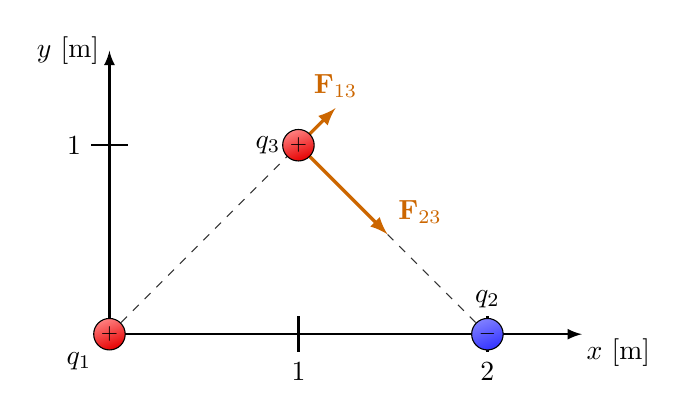
\begin{tikzpicture}
  \def\a{2.4}
  \def\w{0.23}
  \def\R{0.20}
  \def\F{1.4}
  \coordinate (O) at (0,0);
  \coordinate (T) at (\a,\a);
  \coordinate (R) at (2*\a,0);
  
  % AXIS
  \draw[->,thick] (0,0) -- (2.5*\a,0) node[below right=-2] {$x$ [m]};
  \draw[->,thick] (0,0) -- (0,1.5*\a) node[left] {$y$ [m]};
  \foreach \x in {1,2}{
    \draw[thick] (\x*\a,0) ++ (0,+\w) --++(0,-2*\w) node[below] {$\x$};
  }
  \foreach \y in {1}{
    \draw[thick] (0,\y*\a) ++ (+\w,0) --++(-2*\w,0) node[left] {$\y$};
  }
  %\node[below left=3] at (O) {0};
  
  % FORCES
  \draw[dashed,black!80] (O) -- (T);
  \draw[dashed,black!80] (R) -- (T);
  \draw[force] (T) ++ ( 45:\R) --++ ( 45:\F/3) node[above] {$\mathbf{F}_{13}$};
  \draw[force] (T) ++ (-45:\R) --++ (-45:\F)   node[above=8,right] {$\mathbf{F}_{23}$};
  
  % CHARGES
  \draw[charge+] (O) circle (\R) node[scale=0.8] {$+$};
  \draw[charge+] (T) circle (\R) node[scale=0.8] {$+$};
  \draw[charge-] (R) circle (\R) node[scale=0.8] {$-$};
  \node[below left=3] at (O) {$q_1$}; % =+20\,\text{nC}
  \node[left=3]       at (T) {$q_3$}; % =+30\,\text{nC}
  \node[above=6]      at (R) {$q_2$}; % =-10\,\text{nC}
  
\end{tikzpicture}



% ELECTRIC FIELD
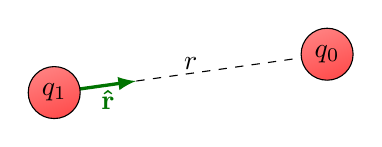
\begin{tikzpicture}
  \def\theta{8}
  \def\r{3.5}
  \def\rh{0.3*\r}
  \coordinate (O) at (0,0);
  \coordinate (R) at (\theta:\r);
  
  \draw[->,dashed] (O) -- (R) node[midway,above=-2] {$r$};
  \draw[vector] (O) ++ (\theta:\R) -- (\theta:\rh) node[midway,below=-2] {$\vu{r}$};
  
  %\draw[->,thick] (0,0) -- (0,1.5*\a) node[left] {$y$ [m]};
  
  % CHARGES
  \draw[charge] (O) circle (\R) node {$q_1$};
  \draw[charge] (R) circle (\R) node {$q_0$};
  
\end{tikzpicture}



\end{document}